\documentclass[]{article}
\usepackage{graphicx}
\usepackage{pgffor}

%opening
\title{CPSC425 A4}
\author{Eric Semeniuc - 54383161}

\begin{document}

\maketitle


\textbf{Q3:}
\foreach \x in {0.40, 0.60, 0.70, 0.75, 0.78, 0.79, 0.80}{
	\textbf{Sift threshold = \x:}\\
	\includegraphics[width=0.8\linewidth]{results/sb_\x_out.png}\\
	\label{fig:Sift threshold = \x}
}

Outlier selection:\\\\
Threshold = 0.4 we have have one outlier in middle\\
Threshold = 0.6 we have one obvious outlier from edge of rice box to trees\\
Threshold = 0.7 another obvious outlier on corner of chair\\
Threshold = 0.75 3 more outliers, 2 on bag (parallel), other on corner of black book\\
Threshold = 0.78 another on edge of bag\\
Threshold = 0.79 1 outlier on bottom of rice box\\
Threshold = 0.8 2 outliers, 1 on chair, 1 in middle of rice box\\\\
A threshold of 0.79 produced the best results while not having more than 10 obvious outliers. It was somewhat important to get the value correct since small increases to the threshold would add many outliers quickly after the ideal threshold

\pagebreak

\textbf{Q4:}\\
\textbf{With Ransac}\\
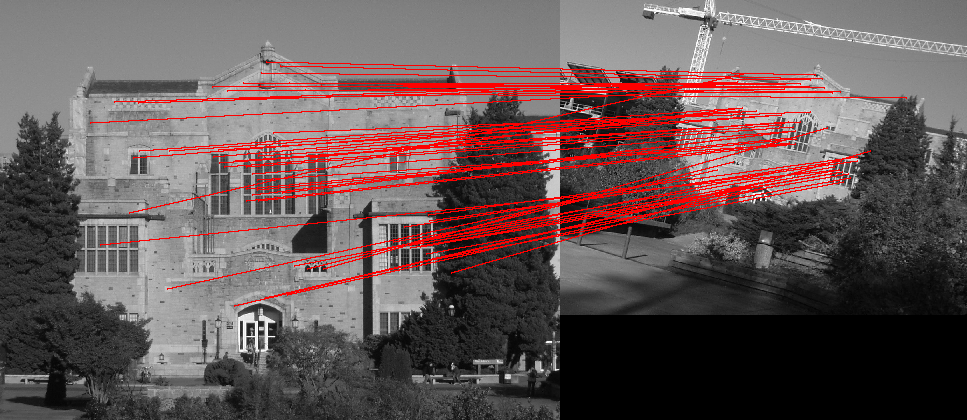
\includegraphics[width=0.8\linewidth]{{results/ll_sift-0.78_orient-0.39_scale-0.40_out}.png}\\
%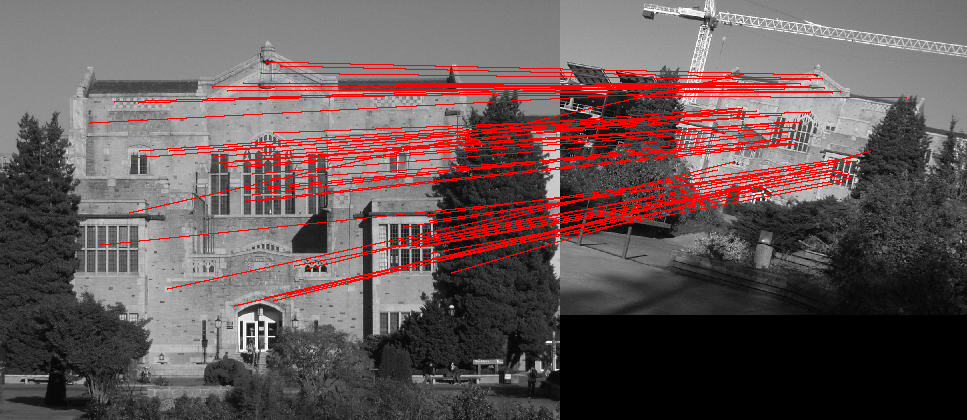
\includegraphics[width=0.8\linewidth]{{results/ll_sift-0.78_orient-0.39_scale-0.45_out}.png}\\
%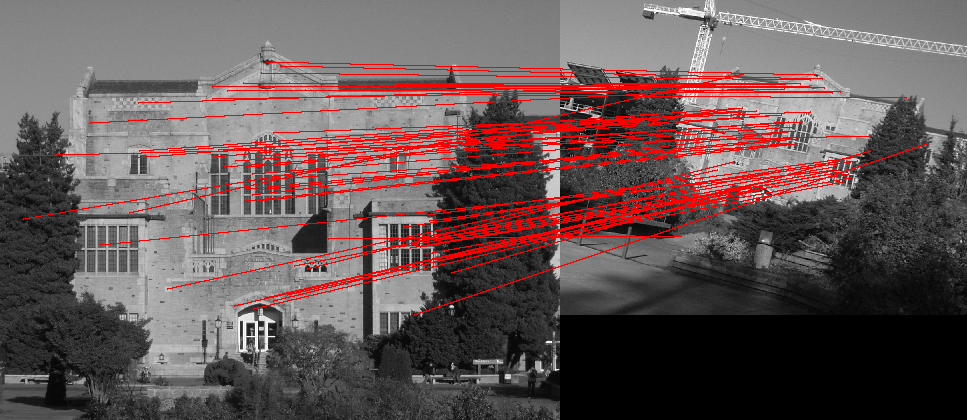
\includegraphics[width=0.8\linewidth]{{results/ll_sift-0.79_orient-0.63_scale-0.45_out}.png}\\
%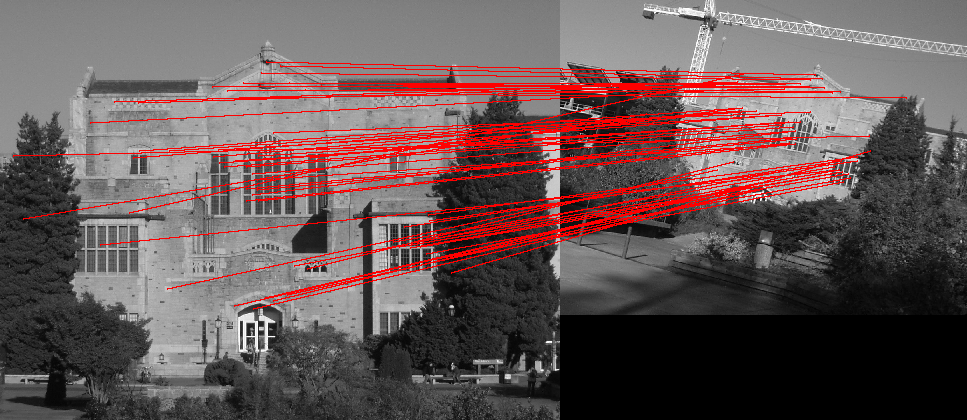
\includegraphics[width=0.8\linewidth]{{results/ll_sift-0.79_orient-0.79_scale-0.50_out}.png}\\
\textbf{No Ransac}\\
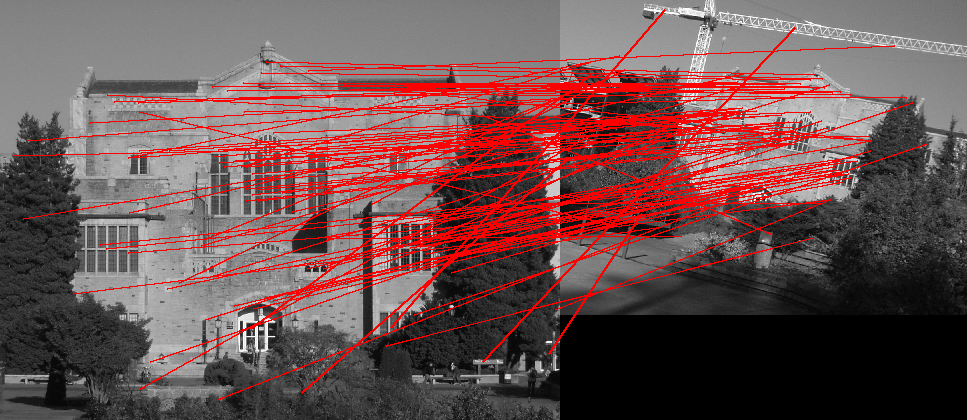
\includegraphics[width=0.8\linewidth]{results/bestNoRansac.png}\\
Best solution was found with SIFT Threshold of 0.78, 0.39 for the orientation threshold, and 0.40 for the scale threshold. The consistency checking allowed us to have more consistent outputs and use higher thresholds in general.
\end{document}
